%%%% $Id: abowd-vilhuber-block-PSD-2012.tex 396 2013-11-03 22:29:27Z lv39 $
%%%% $URL: https://forge.cornell.edu/svn/repos/ncrn-cornell/branches/papers/PSD2012/abowd-vilhuber-block-PSD-2012.tex $
%\documentclass[12pt, conference, compsocconf,onecolumn]{IEEEtran}
%\documentclass[12pt, journal,onecolumn]{IEEEtran}
\documentclass{llncs}
%\IEEEoverridecommandlockouts
% override added by Abowd so that grants could be acknowledged
% Add the compsocconf option for Computer Society conferences.
%

% *** CITATION PACKAGES ***
\usepackage{graphicx}
%\usepackage{natbib}
\usepackage[breaklinks]{hyperref}
\usepackage[printonlyused]{acronym}
\usepackage[usenames]{xcolor}
\usepackage{longtable}
\definecolor{darkblue}{rgb}{0.2,0,0.4}
\definecolor{darkred}{rgb}{0.54,0,0}
\definecolor{light-gray}{gray}{0.95}
\hypersetup{colorlinks=true,linkcolor=black,citecolor=black,urlcolor=black}
%\includeonly{acronyms.tex}
% when preparing the file, also add acronyms.tex to the above list.
% For the final version, this can then be removed.
% *** MATH PACKAGES ***
%
\usepackage[cmex10]{amsmath}
\usepackage[]{bm}
\usepackage{amssymb,latexsym}
% *** SPECIALIZED LIST PACKAGES ***
%
%\usepackage{algorithmic}

% *** ALIGNMENT PACKAGES ***
%
\usepackage{array}

% *** PDF, URL AND HYPERLINK PACKAGES ***
%%%%%%%%%%%%%%%%%%%%%%%%%%%%%%%%%%%%%%%%%%%%%%%%%%%%%%%%%%%%%%%%%%%%%%%%%%%%%%%
% embed files. This can be removed by the editor without loss of functionality
%%%%%%%%%%%%%%%%%%%%%%%%%%%%%%%%%%%%%%%%%%%%%%%%%%%%%%%%%%%%%%%%%%%%%%%%%%%%%%%%
\usepackage{ifpdf}
\ifpdf 
\usepackage{embedfile}
\embedfile{\jobname.tex}
\embedfile{paper.bib}
\embedfile{abstract.tex}
\embedfile{introduction.tex}
\embedfile{main.tex}
\embedfile{discussion.tex}
\embedfile{conclusion.tex}
\embedfile{acronyms.tex}
\embedfile{pie-chart-rdc-data.png}
\embedfile{accesschart.png}
\embedfile{ConfidentialMetadata.png}
\embedfile{abowd-vilhuber-block-PSD-2012.bbl}
\embedfile{abowd-vilhuber-block-PSD-2012.aux}
\embedfile{llncs.cls}
\embedfile{aliascnt.sty}
\fi

\begin{document}
%
% paper title
% can use linebreaks \\ within to get better formatting as desired
\title{A Proposed Solution to the Archiving and Curation of Confidential Scientific Inputs}

% FOR PAPERS, USE THIS VERSION
\author{John~M.~Abowd\inst{1}%
\thanks{Corresponding author: \email{john.abowd@cornell.edu}}%
\and Lars~Vilhuber\inst{1}%
\and William~Block\inst{2}%
}

\institute{Department of Economics and Labor Dynamics Institute, Cornell University, Ithaca, NY, %
 USA \and Cornell Institute for Social and Economic Research, Cornell University, Ithaca, NY, USA}%


%%%%%%%%%%%%%%%%%%%%%%%%%%%%%%%%%%%%%%%%%%%%%%%%%%%%%%%%%%%%%%%%%%%%%%%%%%%%%%%%%
% make the title area
\maketitle

\begin{abstract}
% $Id: abstract.tex 1720 2015-09-25 14:29:12Z lv39 $
% $URL: https://forge.cornell.edu/svn/repos/ncrn-cornell/branches/papers/PSD2014/text/abstract.tex $
The Business Dynamics Statistics is a product of the U.S. Census Bureau that provides measures of business openings and closings,  and job creation and destruction, by a variety of cross-classifications (firm and establishment age and size, industrial sector, and geography). Sensitive data are currently protected through suppression. However, as additional tabulations are being developed, at ever more detailed geographic levels, the number of suppressions increases dramatically. This paper explores the option of providing public-use data that are analytically valid and without suppressions, by leveraging synthetic data to replace observations in sensitive cells. 

\end{abstract}


%% $Id: abstract.tex 1720 2015-09-25 14:29:12Z lv39 $
% $URL: https://forge.cornell.edu/svn/repos/ncrn-cornell/branches/papers/PSD2014/text/abstract.tex $
The Business Dynamics Statistics is a product of the U.S. Census Bureau that provides measures of business openings and closings,  and job creation and destruction, by a variety of cross-classifications (firm and establishment age and size, industrial sector, and geography). Sensitive data are currently protected through suppression. However, as additional tabulations are being developed, at ever more detailed geographic levels, the number of suppressions increases dramatically. This paper explores the option of providing public-use data that are analytically valid and without suppressions, by leveraging synthetic data to replace observations in sensitive cells. 

% For peer review papers, you can put extra information on the cover
% page as needed:
% \ifCLASSOPTIONpeerreview
% \begin{center} \bfseries EDICS Category: 3-BBND \end{center}
% \fi
%
% For peerreview papers, this IEEEtran command inserts a page break and
% creates the second title. It will be ignored for other modes.
%\IEEEpeerreviewmaketitle

\section{Introduction}
% no \IEEEPARstart

%TCIDATA{Version=5.50.0.2960}
%TCIDATA{LaTeXparent=0,0,abowd-vilhuber-PSD-2012.tex}
                      

% $Id: introduction.tex 396 2013-11-03 22:29:27Z lv39 $
% $URL: https://forge.cornell.edu/svn/repos/ncrn-cornell/branches/papers/PSD2012/introduction.tex $

The era of public-use micro-data as a cornerstone of empirical research in
the social sciences is coming to an end---not because it is no longer
feasible to create such data without breaching confidentiality. It still is,
and statistical agencies like the Census Bureau will continue to do so.
Rather, the death knell is being sounded by young scholars pursuing research
programs that mandate inherently identifiable data: geospatial relations,
exact genome data, networks of all sorts, linked administrative records, and
so on. These researchers acquire authorized restricted access to the
confidential, identifiable data and perform their analyses in secure
environments. And their research is challenging fundamental scientific
principles because the restricted access cannot be extended arbitrarily to
the whole user community \cite{Huberman2012}.

The Census Research Data Centers are a leading paradigm for such research,
but other modalities are proliferating rapidly. The researcher is allowed to
publish results that have been filtered through a statistical disclosure
limitation protocol. Scientific scrutiny is hampered because the researcher
cannot effectively implement a data management plan that permits sharing
these restricted-access data with other scholars. In the case of Census RDCs
the relevant statute has been interpreted to prohibit granting long-term
data custody outside of the Bureau except for copies held by the National
Archives, which does not permit public access to these holdings.
University-operated archives like ICPSR may take custody of non-Census
Bureau restricted-access data under some conditions, but they still cannot
freely grant access to the confidential micro-data in their repositories.
The data custody problem is impeding the \textquotedblleft acquire, archive
and curate\textquotedblright\ model that dominated social science data
preservation in the era of public-use micro-data.


\section{Statement of the Problem}

%TCIDATA{Version=5.50.0.2960}
%TCIDATA{LaTeXparent=0,0,abowd-vilhuber-PSD-2012.tex}
                      

% $Id: main.tex 396 2013-11-03 22:29:27Z lv39 $
% $URL: https://forge.cornell.edu/svn/repos/ncrn-cornell/branches/papers/PSD2012/main.tex $
%
% main.tex

\subsection{The Curation of Confidential Data}

In the United States, the \acf{NSF} has required since January 18, 2011 that
all scientific research proposals include a detailed, viable data management
plan, thus recognizing that the acquisition, archival and curation of
scientific data is vital to the integrity of the entire process.\footnote{%
\href{http://www.nsf.gov/eng/general/dmp.jsp}{%
http://www.nsf.gov/eng/general/dmp.jsp} cited on May 20, 2012.} The relevant
test is not \textquotedblleft can the next researcher reproduce current
results,\textquotedblright\ rather it is \textquotedblleft can a researcher
working 50 or 100 years from now recover and correctly re-use the original
data.\textquotedblright\ This standard will be met when ``sufficient information exists with which to understand, evaluate, and build upon a prior work if a third party can replicate the results without any additional information from the author.''  \cite{King1995} 
Libraries have performed the curation (or
preservation) function for millennia. Social scientists recognized the
importance of data management decades ago when the \acf{ICPSR} was formed,
and again a few decades later when \ac{NSF} funded major social science data
initiatives like \ac{IPUMS} at the University of Minnesota and the \acp{RDC}
at the U.S. Census Bureau.

\ac{ICPSR} is now the largest social science data repository in the world
with over 500,000 data sets in its collection, including a growing inventory
of restricted-access datasets.\footnote{%
See \href{http://www.icpsr.umich.edu/icpsrweb/ICPSR/org/index.jsp}{%
http://www.icpsr.umich.edu/icpsrweb/ICPSR/org/index.jsp} , cited on May 20,
2012} IPUMS and IPUMS-International are the definitive sources for household
micro-data originating from population censuses around the world, including
projects for which IPUMS-International is the long-term custodian of a
foreign nation's confidential micro-data.\footnote{%
See \href{https://international.ipums.org/international/about.shtml}{%
https://international.ipums.org/international/about.shtml}, cited on May 20,
2012.} Similar archives, such as the UK Data Archive\footnote{\href{http://www.data-archive.ac.uk/about/archive}%
{http://www.data-archive.ac.uk/about/archive}, accessed May 20, 2012} and
the Australian National Data Service,\footnote{\href{http://www.ands.org.au/}%
{http://www.ands.org.au/}, accessed May 20, 2012} perform similar functions
in other countries. Within statistical agencies, researchers working at the
U.S. Census Bureau and in Census RDCs have acquired and archived a very
substantial collection of micro-data that are now used routinely for
scientific research in economics, sociology, demographics, environmental
science, health, and other fields. Other \ac{NSF}-funded efforts to make
data available have also been very successful.

Figure~\ref{fig:piechart} shows the overall distribution of data sets used
in current and historical RDC projects. It summarizes 1,505 project-dataset
pairs.\footnote{%
Many projects use multiple datasets.} %
%
% Figure Piechart (Figure 1 in NCRN proposal)
\begin{figure}[tbp]
\centering
\caption{Data sets used in U.S. Census Bureau RDC projects}
\label{fig:piechart}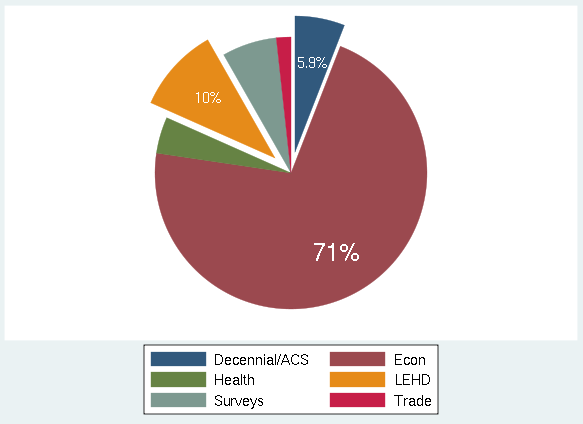
\includegraphics[width=0.5\textwidth]{pie-chart-rdc-data}
\end{figure}
Fully 71\% of all project-datasets use economic (business or establishment)
micro-data. Such data are primarily the establishment-based records from the
Economic Censuses and Surveys, the Business Register, and the \ac{LBD}. With
the exception of the recently-released Synthetic LBD \cite%
{AbowdVilhuber2010,KinneyEtAl2011}, there are no public-use micro-data for
these establishment-based products. Yet, they form the core of the modern
industrial organization studies \cite%
{DunneRobertsSamuelson1989,OlleyPakes1996} as well as modern gross job
creation and destruction in macroeconomics \cite%
{DavisHaltiwangerSchuh,HaltiwangerJarminMiranda2010}.

The next most frequently used data come from the \acf{LEHD} program, a
longitudinally integrated employer-employee database that was created
following a joint Census Bureau-NSF investment in 1999 \cite{AbowdEtAl2009}.
New confidentiality protection methodologies \cite{AbowdEtAl2012,Ashwin2008}
have unlocked large amounts of data for public-use but the structured
metadata has not kept pace. While highly detailed local area tabulations
exist based on the \ac{LEHD} data, no public-use micro-data exist for this
longitudinal job frame or any of its derivative files.

Somewhat surprisingly, only about 6\% of the project-dataset pairs involve
confidential Decennial/American Community Survey (ACS) data. Public-use
decennial files from both the long and short forms have existed for decades.
These lacked geographical detail when they were based on the old long form.
However, geographically detailed historical census and ACS files are now
part of the Census RDC-accessible micro-data collection. Thus, one can
reasonably speculate that the fraction of projects that use confidential %
\ac{ACS} will rise in the coming years.

Over the course of the last decade a framework for providing access to the
confidential micro-data that form the basis for the Census Bureau's major
data products has emerged. This framework is consistent with the statutory
obligations of the Bureau's co-custodians; namely, that research use of the
micro-data be consistent with the enabling legislation for each constituent
data source and that the appropriate administrative review occur prior to
the onset of new research. This framework is currently the best available
political compromise in the United States, but it can be considered neither
permanent nor durable.

A similar spectrum of data access protocols has emerged in Europe. They
range from relatively easy research access to confidential micro-data to
remote processing of firm or person micro-data\footnote{%
See for instance \href{http://www.bancaditalia.it/statistiche/indcamp/sondaggio/bird}%
{http://www.bancaditalia.it/statistiche/indcamp/sondaggio/bird} and \href{http://www.lisproject.org/data-access/lissy.htm}%
{http://www.lisproject.org/data-access/lissy.htm} accessed May 20, 2012.} to
simple online tabulators at most statistical agencies. As of 2012, efforts
are underway to harmonize European \cite{Bujnowska2012} or international 
\cite{Lunati2012} regulations, facilitating a standardized approach to
cross-national data access. However, it appears that most efforts have
concentrated on technical and legal questions.

To the extent that the next generations of social scientists build their
careers on the basis of original discoveries emanating from these
confidential data in the United States and elsewhere, a regulatory consensus
must emerge that treats the underlying confidential data as a vital
scientific asset, including its curation procedures.

When this consensus emerges, it will be too late to begin the curation
process. In contrast to printed data (otherwise known as books and
journals), which have unique handles (\ac{ISBN} and \ac{ISSN} are almost
universally applied), data files generally have not yet been managed in a
similar fashion.\footnote{%
To the best of our knowledge, only \ac{ICPSR} and the UK Data Archive assign
unique \acp{DOI}, but only to data that they physically control.} Part of
the problem, of course, is that while the origin and version of printed
matter used to be easily identifiable (expensive print runs and distribution
paths ensured that no book ever got to its 500th edition), data have become
more and more variable and extensible. Thus, most data currently lack a
unique handle that can be used to trace their design, provenance and vintage.

\subsection{Current Archive Model Fails}

Big data archives such as \ac{ICPSR}, \ac{IPUMS}, the UK Data Archive, or
the International Data Service Center at IZA have done an extraordinary job
of preserving public-use data--often rescuing them from oblivion--and
provide some idiosyncratic way to refer to specific samples. But there is a
fundamental, and critical, difference between the approach taken by the data
archives as compared to the approach taken by the U.S. Census Bureau, other
governmental agencies and most private organizations that use confidential
micro-data as the basis for original research or provide research access to
such data. The curation function is either absent or woefully neglected.
Consequently, there is a substantial risk of breach of the scientific
integrity of the research process itself because the findings that are
reported in the peer-reviewed journals are based on analyses of the
confidential restricted-access data, but only public-use data are released
for open scrutiny. It is the confidential data themselves that must be
curated, not just the disclosure-limited public-use products that this
research produces, in order to afford future generations of scientists the
same ability to scrutinize this work as many generations have had for work
based on the major public-use data products developed in the last 50 years.%
\footnote{%
The 1960 U.S. Census of Population and Housing Public Use Micro Sample,
released in 1963, was the first such product released by a national
statistical agency \cite{Ruggles1991}.} The statutory custodians of the
restricted-access data, in most cases government agencies but also
private-sector entities, need substantial help from the scientific community
in order to ensure that vital research data they have now acquired are
properly curated.

The problem has been caused by a subtle but pervasive barrier to effective
application of current best-practice long-term data management systems. When
conventional repositories like ICPSR, IPUMS-International and the IZA\ Data
Enclave have attempted to apply the acquisition, archive and curation
processes developed for public-use data directly to restricted-access data,
the management of restricted-access data adds an additional layer, sometimes
called stewardship, to the accepted practices. The data archive takes
physical custody of a certified-true copy of the confidential data under the
terms of a restricted-access data provider agreement with the statutory
custodian. This agreement establishes the statutory custodian's legal
authority to grant physical data custody to the archive and delineates the
terms and conditions of future use, including any disclosure limitation
protocols that must be used. At the same time, the archive acquires or
creates the metadata that are essential to the curation process. From this
point forward, management of the restricted-access data is very similar to
management of public-use data. In particular, many resources from the data
archive and the research community can be used to enhance the curation
process.

But if the conventional archive cannot take long-term custody of the
original data, this model fails because it does not have a mechanism for
synchronizing the provenance and metadata histories applicable to the
confidential data that can be audited and verified by future data users. The
U.S. Census Bureau and many other American government agencies are
prohibited by statute from granting an archive like ICPSR or IPUMS long-term
physical custody of their confidential data. Private-sector entities may
also have legal barriers emanating from data privacy promises, or may simply
hesitate to provide potential competitors access to detailed micro-data.
Both micro-data and metadata are locked up and inaccessible.

Because private entities like Microsoft or Google and government agencies
like the U.S. Census Bureau retain custody of both the confidential data and
critical metadata, a substantially modified curation protocol is required to
ensure that the actual inputs to published research are preserved. Some
requirements for this protocol are discussed here.


\section{Principles for Solution}

%TCIDATA{Version=5.50.0.2960}
%TCIDATA{LaTeXparent=0,0,abowd-vilhuber-PSD-2012.tex}
                      

% -*- latex -*-
%
% Time-stamp: <02/03/14 16:29:52 vilhuber>
%              Automatically adjusted if using Xemacs
%              Please adjust manually if using other editors
%
%

\subsection{The Commitment of Primary Custodians}

\begin{figure}[tbp]
\centering
\caption{The Parallel Problems of Public and Private Data Stewards}
\label{fig:accesschart}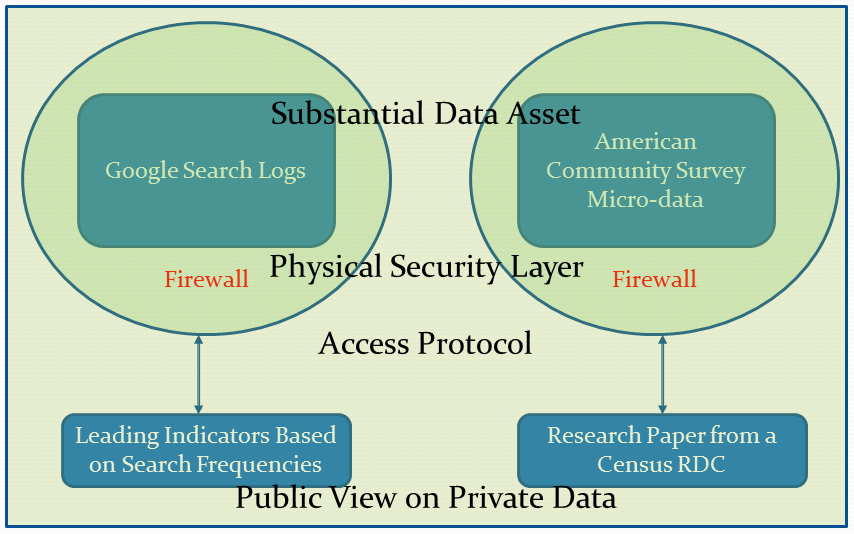
\includegraphics[width=0.5\textwidth]{accesschart}
\end{figure}

Figure \ref{fig:accesschart} shows the problem faced by public or private
data custodians who grant research access to their data. The primary data
asset is protected by both a physical security layer and an access protocol,
both of which stand between the ultimate user of the scientific output and
the confidential data. The physical security layer ensures that other
potential users do not gain unauthorized access. The access protocol limits
what may be released and published using privacy-preserving or statistical
disclosure limitation methods.

Unless the primary custodian commits to long-term archival and curation of
both the data and their metadata, the integrity of the process is corrupted.
In the private domain, future users of the published indicator cannot rely
upon the continued scrutiny of other users to expose and correct defects in
the inputs and methodology of the published indicators. In the public
domain, users of the research output cannot properly review the original
work nor reliably build on it in future work. Both failures result from the
effective denial of access to both the curated data and metadata.

Once a private or public provider commits to the long-term obligations of
scientific data custodian, the problem becomes how to integrate the archival
and curation process with their physical security layer and access
protocols. This integration is an unsolved problem although tools from both
statistical disclosure limitation and data curation are useful.

\subsection{Transparency among Users}

All of the data processing for the scientific research referenced in Figure %
\ref{fig:accesschart} is done in a controlled environment that lacks the
tools needed to conform to emerging standards for data documentation.
\textquotedblleft \lbrack T]he metadata of data files are crucial for
browsing and searching\textquotedblright\ because data files generally do
not lend themselves to the same indexing techniques as text files \cite%
{hensequadt2011}. %\marginpar{BB2 originally appeared here}
The consequence is data that are difficult to discover,
and, when found, only sparsely documented. Researchers waste valuable time
trying to determine the content and structure of confidential datasets in
sufficient detail to support their proposed secondary analysis. Some
confidential datasets even contain variables whose names themselves are
masked.\footnote{%
For example, the U.S. Census Bureau's establishment micro-data contain data
elements from the Internal Revenue Service whose confidentiality stewards
have designated the names of certain fields as \textquotedblleft official
use only,\textquotedblright\ which implies that these metadata are
confidential too.} When confronted with difficult problems such as these,
researchers resort to time-consuming alternative search strategies like
email queries.

A better solution is needed, one that allows researchers to efficiently
learn about and work with the confidential data without violating existing
access protocols, and one that ensures that the exact historical research
inputs and their provenance are curated for a long time.  Inefficiencies that
current users might be prepared to tolerate discourage potential users from
ever starting. The absence of reliable curation may effectively orphan the
research done in this early era of restricted-access data use.


\subsection{Conformance to Standards}

\begin{figure}[tbp]
\centering
\caption{Example of Confidential and Derived Public-use Metadata}
\label{fig:ConfidentialMetadata}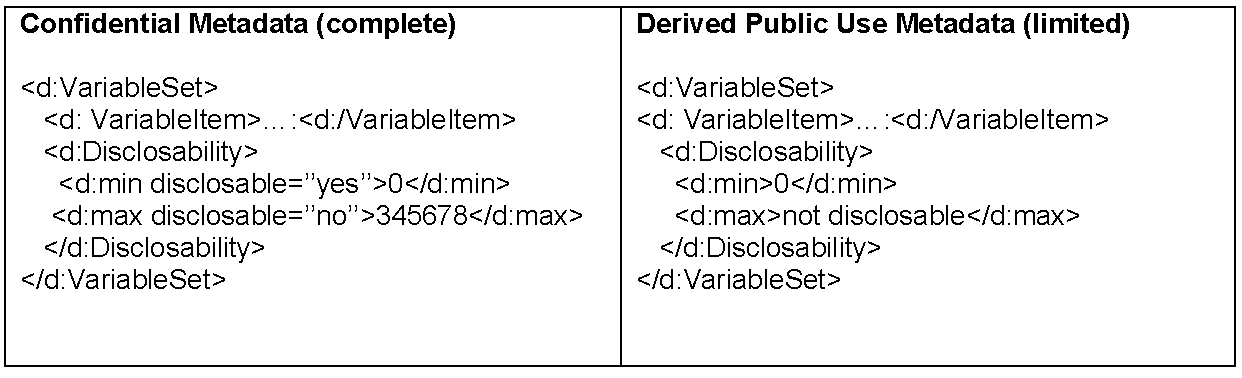
\includegraphics[width=0.5%
\textwidth]{ConfidentialMetadata}
\end{figure}

%BB2 
%\marginpar{BB2 moved here}
The Royal Society \cite{RoyalSociety2012} has recently called for metadata that goes beyond basic, generic contextual information and meets four fundamental characteristics.  Metadata must be:  accessible (a researcher can easily find it); intelligible (to various audiences); assessable (are researchers able make judgments about or assess the quality of the data); and usable (at miniumum, by other scientists). 

Leading metadata standards such as the \ac{DDI} and \ac{SDMX} are flexibly
designed to ingest documentation from a variety of source files. Using these
tools to standardize the curation of confidential research data permits the
exercise to benefit from the same technological innovations that open-access
data archives already use. \cite{GregoryHeus2007,BlankRasmussen2004}   %\marginpar{BB3}

But the benefits go in both directions. These tools need to be extended so
that they can naturally accommodate metadata items that respect
privacy-preserving and statistical disclosure limitation procedures. In a
model based on \ac{XML}, for example, this might be done through the
addition of machine-actionable attributes to elements describing variables.
An example of a possible template, assuming an \ac{XML}-like structure, is
shown in Figure \ref{fig:ConfidentialMetadata}. The example could be
applied, for instance, to a variable containing data on income or sales. The
element \textquotedblleft Disclosability\textquotedblright\ is not currently
present in the \ac{DDI} specification, but could be defined in a future
release.

The full-information metadata can be presented through a restricted-access
website available only within the secure environment itself, running the
same web frontend used for the public interface. Such a development itself
would provide a major advance in the ability of confidential data
researchers to conduct their work because in many environments, including
those supported in U.S. Census Bureau RDCs, the public metadata interface
cannot be viewed inside the secure layer and the confidential data have not
been curated to the same level of specificity.

\subsection{Training of Future Users}

Graduate social science programs and their faculties haven't worried about
how future users would gain adequate instruction in the major public-use
micro-datasets for decades. The body of discipline-specific capital is
sufficiently extensive and the data curation tools sufficiently advanced,
that doctoral programs and social science faculty members can rely on course
assignments, specialized workshops, and existing archives and repositories
to disseminate such methods. That doesn't happen with confidential data
because the potential user must usually already have a specific approved
project and be allowed access inside the security protocol layer before any
study of the metadata or analysis of the actual data can be done.

These costs are sometimes mitigated by virtual enclaves like the Cornell
VirtualRDC\footnote{%
See \href{http://www.vrdc.cornell.edu/news/}{%
http://www.vrdc.cornell.edu/news/} cited on May 20, 2012.}, the NORC\ Data
Enclave\footnote{%
See \href{http://www.dataenclave.org/index.php/home/welcome}{%
http://www.dataenclave.org/index.php/home/welcome} cited on May 20, 2012.},
or the \ac{IDSC} of the \ac{IZA}.\footnote{%
See \href{http://idsc.iza.org/}{http://idsc.iza.org/} cited on May 20, 2012}
But usually the fixed costs are simply too high to incorporate this kind of
hands-on experience in regular doctoral courses or short-term research
projects. The existence of coordinated metadata curation, as described
above, mitigates this difficulty by providing a layer of access outside of
the secure protocol for the metadata that supports the research outputs.


\section{Conclusion}

In this paper, we have described two alternate mechanisms to substitute for suppressions in  small-cell tabulations of business 
microdata, with the goal of improving analytic validity while maintaining a sufficiently high 
standard of disclosure limitation. Neither mechanism fundamentally changes the existing suppression methodology, rather, the mechanisms work to fill in the holes created by the suppression methodology. 

Leveraging the availability of a high-quality synthetic datasets 
(the Synthetic LBD) with proven disclosure limitation efficiency and analytic validity \cite{KinneyEtAl2011}, the first 
method is very simple, but may suffer from seam biases and time-inconsistency. The second 
method aims to improve on that by ``blending in'' synthetic establishments, which may slightly 
reduce analytic validity in time periods where the strict application of the suppression 
algorithms would no longer impose any constraints, but improving on the time-series properties 
of the released data. 

Several limitations of the research presented here should be highlighted. The examples provided in this article rely on an earlier release of the Synthetic LBD 
\cite{KinneyEtAl2011}. Recent developments to improve the micro-level analytic validity of the 
\ac{SynLBD} \cite{CES-WP-2014-12} should improve the analytic validity of the mechanisms 
proposed here as well.  We also compare our proposed mechanisms to the actual published, but otherwise unmodified \ac{BDS}. Comparing to post-publication improvements to a table with suppressions \cite{HolanEtAl2010} will inevitably lead to an apparent reduction in the utility of this particular approach. Finally, the approach relies on continuous availability of synthetic microdata with analytical validity. Other approaches rely on fewer data points, and thus be favored due to lower implementation costs.

Future work for this paper involves assessing the procedure on a wider variety of variables, better synchronisation of the computational algorithms underlying the BDS and the SynBDS, and improved assessment at the microdata level of the protection afforded by Algorithm~1.







% use section* for acknowledgement
\section*{Acknowledgment}

We acknowledge NSF grants SES 9978093, ITR 0427889, SES 0922005, SES 1042181, and SES 1131348.

\bibliography{abbrev,paper}
%\bibliographystyle{IEEEtranS}
\bibliographystyle{splncs_srt}

\section*{Acronyms used}

%TCIDATA{Version=5.00.0.2570}
%TCIDATA{LaTeXparent=0,0,sw-edit.tex}

% $Id: acronyms.tex 1720 2015-09-25 14:29:12Z lv39 $
% $URL: https://forge.cornell.edu/svn/repos/ncrn-cornell/branches/papers/PSD2014/text/acronyms.tex $
%
% Define acronyms to be used in the text here. See
% http://www.mackichan.com/index.html?techtalk/456.htm~mainFrame for usage in
% Scientific workplace context

\begin{acronym}
\acro{ACS}{American Community Survey} 
\acro{AHEAD}{Study of Assets and Health Dynamics Amongst the Oldest Old}
\acro{ASCII}{American Standard Code for Information  Interchange} %, typically used to denote raw text files in PC or Unix environments
\acro{ASM}{Annual Survey of Manufacturers}
\acro{BDS}{Business Dynamics Statistics}
\acro{BED}{Business Employment Dynamics}
\acro{BES}{Business Expenditure Survey}
\acro{BLS}{Bureau of Labor Statistics}
\acro{BRB}{Business Register Bridge}
\acro{BR}{Business Register}
\acro{CAC}{Cornell Center for Advanced Computing}
\acro{CBP}{County Business Patterns}
\acro{CBSA}{Core-Based Statistical Area}
\acro{CER}{Covered Earnings Records}
\acro{CES}{Center for Economic Studies}
\acro{CEW}{Covered Employment and Wages}%. Employment statistics program run by BLS in  conjunction with all states, also known as ES-202. Generally, when used  in this document, refers to public-use tabulations from the CEW, as  opposed to the confidential microdata received directly from the states.
\acro{CISER}{Cornell Institute for Social and Economic Research}
\acro{CIT}{Cornell Information Technologies}
\acro{CODA}{Children of Depression}
\acro{CPI}{Consumer Price Index}
\acro{CPI-U}{Consumer Price Index (All Urban Consumers)}
\acro{CPR}{Composite Person Record}
\acro{CPS}{Current Population Survey}
\acro{CRADC}{Cornell Restricted Access Data Center}
\acro{CTC}{Cornell Theory Center}
\acro{DCC}{Data Confidentiality Committee}
\acrodef{err}{excess reallocation rate}
\acrodef{jcr}{job creation rate}
\acrodef{jdr}{job destruction rate}
\acrodef{jrr}{job reallocation rate}
\acrodef{wrr}{worker reallocation rate}
\acro{DER}{Detailed Earnings Record}
\acro{DRB}{Disclosure Review Board}
\acro{DWS}{Displaced Worker Supplement}
\acro{ECF}{Employer Characteristics  File}
\acro{EHF}{Employment History Files}
\acro{EIN}{\acroextra{(federal) }Employer Identification Number}
\acro{ERR}{Excess Reallocation Rate}
\acro{ES-202}{ES-202\acroextra{. An older name for the \ac{QCEW} program}}
\acro{FHFA}{Federal Housing Finance Agency}
\acro{FIPS}{Federal information processing standards codes\acroextra{\ issued     by \ac{NIST}}}
\acro{FTI}{Federal Tax Information\acroextra{, typically covered under     Title 26, U.S.C.}}
\acro{GAL}{Geocoded Address List}
\acro{GIS}{Geographic Information System}
\acro{HPI}{House Price Index}
\acro{HRS}{Health and Retirement Study}
\acro{ICF}{Individual Characteristics File}
\acro{IRB}{Institutional Review Board}
\acro{IRS}{Internal Revenue Service}
\acro{ISR}{Institute for Social Research}
\acro{JCR}{Job Creation Rate}
\acro{JDR}{Job Destruction Rate}
\acro{JOLTS}{Job Openings and Labor Turnover Survey}
\acro{JRR}{Job Reallocation Rate}
\acro{LAUS}{Local Area Unemployment Statistics}
\acro{LBD}{Longitudinal Business Database}
\acro{LDB}{\ac{BLS}'s Longitudinal Business Database}
\acro{LED}{Local Employment Dynamics}
\acro{LEHD}{Longitudinal Employer-Household Dynamics}
\acro{LMI}{Labor Market Information}
\acro{MBR}{Master Beneficiary Record}
\acro{MEF}{Master Earnings File}
\acro{MER}{Master Earnings Record}
\acro{MLS}{Mass Layoff Statistics}
\acro{MMS}{Methodology, Measurement, and Statistics}
\acro{MN}{Minnesota}
\acro{MSA}{Metropolitan Statistical Area}
\acro{MSD}{Metropolitan Statistical Division}
\acro{MWR}{Multiple Worksite Report}
\acro{NAICS}{North American Industry Coding System}
\acro{NECTA}{New England  City and Town Area}
\acro{NIA}{National Institute on Aging}
\acro{NIST}{National Institute of Standards and Technology}
\acro{NLSY}{National Longitudinal Study of Youth}
\acro{NSF}{National Science Foundation}
\acro{NSTA}{NAICS SIC Treatment of Auxiliaries}
\acro{OTM}{OnTheMap}
\acro{PCF}{Person Characteristics File}
\acro{PHF}{Person History File}
\acro{PIK}{Protected Identity Key}
\acro{PSID}{Panel Study of Income Dynamics}
\acro{QCEW}{Quarterly Census of Employment and Wages\acroextra{, managed by   the \acf{BLS}}}
\acro{QWI}{Quarterly Workforce Indicators}
\acro{RDA}{Restricted Data Application}
\acro{RDC}{Research Data Center}
\acro{RUN}{Reporting unit number}
\acro{SEIN}{State employer identification number\acroextra{. It is     constructed from the state \ac{FIPS} code and the UI account     number. The BLS refers to the UI account number in combination with the     reporting unit number as SESA-ID}}
\acro{SEINUNIT}{SEIN reporting unit}
\acro{SEPB}{Summary of Earnings and Projected Benefits} % confidential SSA                                % file
\acro{SESA-ID}{State Employment Security Agency ID\acroextra{. The UI     account number in combination with the Reporting Unit Number is treated   as a unique establishment identifier.}}
\acro{SESA}{State Employment Security Agency}
\acro{SIC}{Standard Industry Classification}
\acro{SIPP}{Survey of Income and Program Participation}
\acro{SLID}{Survey of Labour and Income Dynamics}
\acro{SPF}{Successor-Predecessor File}
\acro{SRMI}{Sequential Regression Multiple Imputation}
\acro{SSA}{Social Security Administration}
\acro{SSI}{Supplemental Security Income}
\acro{SSN}{Social Security Number}
\acro{SSR}{Supplemental Security Record}
\acro{SynLBD}{Synthetic \ac{LBD}\acroextra{, a synthetic microdata file at the establishment level}}
\acro{U2W}{Unit-to-Worker Impute}
\acro{UI}{Unemployment Insurance}
\acro{WB}{War Babies}
\acro{WIA}{Workforce Investment Act}
\acro{WIB}{Workforce Investment Board}
\acro{WRR}{Worker Reallocation Rate}
\acro{WTS}{Windows Terminal Services}

% Usage in the later text:
%  \ac{acronym}         Expand and identify the acronym the first time; use
%                       only the acronym thereafter 
%  \acf{acronym}        Use the full name of the acronym.
%  \acs{acronym}        Use the acronym, even before the first corresponding
%                       \ac command 
%  \acl{acronym}        Expand the acronym without using the acronym itself.
\end{acronym}

%%% Local Variables: 
%%% mode: latex
%%% TeX-master: "proposal"
%%% End: 

\begin{verbatim}
$Date: 2013-11-03 17:29:27 -0500 (Sun, 03 Nov 2013) $ 
$Rev: 396 $ 
$Author: lv39 $
\end{verbatim}
{\footnotesize
This document contains its component \LaTeX \ files embedded/attached.}
\end{document}
